\documentclass[a4paper]{article}
\usepackage[utf8]{inputenc}
\usepackage[T1]{fontenc}
\usepackage{graphicx}
\usepackage{hyperref}
\usepackage[ngerman]{babel}
\usepackage{fancyhdr}
\usepackage{xurl}
\usepackage{titling}

\newcommand{\bardots}{\smash{\parbox[b]{1.2em}{\rule{1.2em}{0.2ex}\\[-1ex]\dots}}}
\newcommand{\justbar}{\smash{\parbox[b]{1.2em}{\rule{1.2em}{0.2ex}\\[-1ex]\phantom{\dots}}}}
\newcommand{\justdots}{\smash{\parbox[b]{1.2em}{\dots}}}

\newcommand{\CustomTitle}[9]{
    \thispagestyle{empty}
    \vspace*{\stretch{1}}
    {\parindent0cm \rule{\linewidth}{.7ex}}
    \begin{flushright}
        \vspace*{\stretch{1}}
        \sffamily\bfseries\huge
        #1\\
        \vspace*{\stretch{1}}
        \sffamily\bfseries\small
        #2\\
        \vspace*{\stretch{1}}
        \sffamily\bfseries\small
        #3
    \end{flushright}
    \rule{\linewidth}{.7ex}

    \vspace*{\stretch{1}}
    \begin{center}
        
\includegraphics[width=2in]{Resources/Logo.png} \\
        \vspace*{\stretch{1}}
        \textbf{\Large Dokumantation}\\

        \vspace*{\stretch{2}}
        \textbf{\large Informatik}\\
        \textbf{\large Klasse 4AT}

        \vspace*{\stretch{1}}
        \textbf{\large Professor: Rainer Ulrich}  \\[1mm]

        \vspace*{\stretch{1}}
        \textbf{\large Brixen, den 03. Mai 2023}\\
        \vspace*{\stretch{0.25}}
    \end{center}
}

\pagestyle{fancy}
\fancyhf{}
\fancyhead[L]{Grafischer Darstellungsrechner}
\fancyfoot[C]{\thepage}
\renewcommand{\headrulewidth}{0.4pt}

\begin{document}

\CustomTitle
{Grafischer Darstellungsrechner}
{Authors: Priller Patrick, Mairhofer David, Pernthaler Daniel}
{\href{mailto:stpripat@bx.fallmerayer.it}{stpripat@bx.fallmerayer.it}, \href{mailto:stmaidav@bx.fallmerayer.it}{stmaidav@bx.fallmerayer.it}, \href{mailto:stperdan@bx.fallmayer.it}{stperdan@bx.fallmerayer.it}}

{Oberschulzentrum J. Ph. Fallmerayer}
{Brixen}
{\today}
{Rainer Ulrich}
{}

\clearpage

\lhead{}
\pagenumbering{arabic}
\setcounter{page}{1}
\lhead{Grafischer Darstellungsrechner}
\tableofcontents

\clearpage

\section{Themenbeschreibung}

\subsection{Projektziele}

In diesem Projekt verfolgen wir das Ziel, eine benutzerfreundliche und leistungsfähige grafische Funktionen-Plotting-Anwendung zu entwickeln, die es Benutzern ermöglicht, mathematische Funktionen und ihre Ableitungen zu visualisieren und zu analysieren. Um dieses Ziel zu erreichen, haben wir uns folgende spezifische Ziele gesetzt:

\begin{itemize}
\item Entwicklung einer benutzerfreundlichen Oberfläche, die es Benutzern ermöglicht, Funktionen einfach einzugeben und zu bearbeiten.
\item Unterstützung einer breiten Palette von mathematischen Funktionen, einschließlich linearer, quadratischer, exponentieller und trigonometrischer Funktionen.
\item Integration von APIs wie mxParser und JScience, um die Funktionalität und Benutzerfreundlichkeit der Anwendung zu erweitern.
\item Implementierung von Funktionen zur Berechnung und Anzeige von Ableitungen und Kurvendiskussionen.
\item Bereitstellung von Werkzeugen zur Anpassung der Darstellung von Funktionen und des Plotbereichs.
\item Ermöglichung von Zoomen und Verschieben des Plotbereichs, um die Anzeige von Funktionen flexibel zu gestalten.
\item Entwicklung eines effektiven Testverfahrens, um sicherzustellen, dass die Anwendung korrekt funktioniert und benutzerfreundlich ist.
\item Erstellung einer umfassenden Dokumentation, die den Entwicklungsprozess, die Systemarchitektur und die Benutzung der Anwendung beschreibt.
\end{itemize}

Durch das Erreichen dieser Ziele wollen wir eine leistungsstarke und benutzerfreundliche Plotter-Anwendung schaffen, die sowohl für den Bildungsbereich als auch für professionelle Anwender wertvoll ist und die Visualisierung und Analyse von mathematischen Funktionen vereinfacht.


\subsection{Unsere Vision}
Unsere Vision für das Plotter-Projekt war es, eine benutzerfreundliche und leistungsfähige Java-basierte grafische Funktionen-Plotting-Anwendung zu entwickeln, die es Benutzern ermöglicht, mathematische Funktionen und ihre Ableitungen zu visualisieren. Wir wollten eine breite Palette von Funktionen unterstützen, einschließlich linearer, quadratischer, exponentieller und trigonometrischer Funktionen. Dabei sollte die Anwendung die mxParser-Bibliothek verwenden, um mathematische Ausdrücke zu analysieren und ihre Werte zu berechnen.

Zu Beginn des Projekts haben wir uns darauf konzentriert, die Kernfunktionen der Anwendung zu entwickeln, wie das Plotten von Funktionen in einer benutzerfreundlichen Oberfläche, das Berechnen und Anzeigen von Ableitungen von Funktionen, das Anwenden von Konstanten und Variablen auf Funktionen, das Ein- und Ausblenden von Funktionen im Graphen und das Anpassen des Erscheinungsbilds des Plotbereichs. Zudem haben wir die Möglichkeit geschaffen, die Ansicht des Plotbereichs zu vergrößern und zu verkleinern.

Wir wollten sicherstellen, dass die Anwendung einfach zu installieren und auszuführen ist, weshalb wir uns für den Einsatz von Maven zur Erstellung des Projekts entschieden haben. Um das Projekt schnell und einfach zu nutzen, haben wir detaillierte Anweisungen zur Installation der erforderlichen Abhängigkeiten, zum Erstellen des Projekts mit Maven und zum Ausführen der Anwendung bereitgestellt.

Insgesamt war unsere Vision, ein leistungsstarkes und benutzerfreundliches Plotter-Tool zu entwickeln, das sowohl für den Bildungsbereich als auch für professionelle Anwender wertvoll ist und die Visualisierung und Analyse von mathematischen Funktionen vereinfacht.

\subsection{Potenziell nutzbare APIs}

In unserem Plotter-Projekt haben wir verschiedene APIs in Betracht gezogen, um die Funktionalität und Benutzerfreundlichkeit der Anwendung zu erweitern. Zwei der vielversprechendsten APIs, die wir untersucht haben, sind mxParser und JScience.

\subsubsection{mxParser}

mxParser ist eine vielseitige und leistungsfähige Bibliothek zur Analyse und Berechnung mathematischer Ausdrücke. Die Bibliothek ist in Java geschrieben und unterstützt eine breite Palette von Funktionen, einschließlich algebraischer, trigonometrischer, exponentieller und logarithmischer Funktionen. Wir haben mxParser in unserem Plotter-Projekt verwendet, um mathematische Ausdrücke zu analysieren und ihre Werte zu berechnen. Die offizielle Website von mxParser bietet umfassende Dokumentation und Beispiele zur Verwendung der Bibliothek: \url{http://mathparser.org/}

\subsubsection{JScience}

JScience ist eine umfangreiche Java-Bibliothek, die verschiedene wissenschaftliche Disziplinen abdeckt, darunter Mathematik, Physik, Chemie und Informatik. Die Bibliothek bietet eine Reihe von Funktionen, die für unser Plotter-Projekt nützlich sein könnten, wie z.B. Unterstützung für komplexe Zahlen, Einheitenkonversion und lineare Algebra. JScience könnte verwendet werden, um die Funktionalität unserer Anwendung zu erweitern und die Unterstützung für zusätzliche mathematische Funktionen und Operationen zu verbessern. Weitere Informationen zu JScience finden Sie auf der offiziellen Website: \url{http://jscience.org/}\\

Durch die Integration dieser APIs in unser Plotter-Projekt können wir die Benutzererfahrung und die Funktionalität unserer Anwendung weiter verbessern und eine breitere Palette von mathematischen Funktionen und Operationen unterstützen.

\newpage

\subsection{Technologien und Tools}

Bei der Entwicklung des Plotters haben wir eine Reihe von Technologien und Tools verwendet, um eine solide und benutzerfreundliche Anwendung zu erstellen. In diesem Abschnitt werden die wichtigsten Technologien und Tools vorgestellt, die wir im Projekt eingesetzt haben:

\subsection{Programmiersprache und Plattform}

\begin{itemize}
\item \textbf{Java}: Wir haben uns für die Programmiersprache Java entschieden, da sie plattformübergreifend, objektorientiert und gut geeignet für die Entwicklung von grafischen Anwendungen ist. Java bietet eine breite Palette von Bibliotheken und Frameworks, die die Implementierung der benötigten Funktionen erleichtern.

\item \textbf{JavaFX}: Für die Erstellung der grafischen Benutzeroberfläche haben wir JavaFX verwendet, ein modernes Framework für die Entwicklung von Desktop-Anwendungen in Java. JavaFX ermöglicht die Erstellung von ansprechenden und interaktiven Benutzeroberflächen und bietet viele nützliche UI-Komponenten, die für unser Projekt relevant sind.
\end{itemize}

\subsection{APIs und Bibliotheken}

\begin{itemize}
\item \textbf{mxParser}: Diese leistungsfähige Bibliothek wird verwendet, um mathematische Ausdrücke zu analysieren und ihre Werte zu berechnen. mxParser unterstützt eine Vielzahl von Funktionen, was es uns ermöglicht, eine breite Palette von mathematischen Funktionen in unserer Anwendung zu unterstützen.

\item \textbf{JScience}: JScience ist eine umfangreiche Java-Bibliothek, die verschiedene wissenschaftliche Disziplinen abdeckt. Durch die Integration von JScience in unser Projekt könnten wir die Funktionalität unserer Anwendung erweitern und zusätzliche mathematische Funktionen und Operationen unterstützen.
\end{itemize}

\subsection{Entwicklungsumgebung und Tools}

\begin{itemize}
\item \textbf{IntelliJ IDEA}: Wir haben die IntelliJ IDEA-Entwicklungsumgebung verwendet, um unseren Code zu schreiben, zu testen und zu debuggen. IntelliJ IDEA bietet eine Vielzahl von Funktionen, die die Entwicklung von Java- und JavaFX-Anwendungen erleichtern, einschließlich Code-Vervollständigung, Refactoring-Tools und Integration mit Versionskontrollsystemen wie Git.

\item \textbf{Maven}: Maven ist ein Build-Management-Tool, das wir verwendet haben, um den Build-Prozess zu automatisieren und die Abhängigkeiten unseres Projekts zu verwalten. Maven erleichtert die Integration von externen Bibliotheken wie mxParser und JScience und stellt sicher, dass unser Projekt auf verschiedenen Plattformen und Systemen konsistent gebaut und ausgeführt werden kann.

\newpage

\item \textbf{Git}: Für die Versionskontrolle und das Teamwork haben wir Git verwendet. Git ermöglicht es uns, Änderungen am Code nachzuvollziehen, verschiedene Versionen der Anwendung zu verwalten und die Zusammenarbeit zwischen Teammitgliedern zu erleichtern.
\end{itemize}

Durch die Kombination dieser Technologien und Tools konnten wir eine leistungsfähige und benutzerfreundliche Anwendung entwickeln, die es Benutzern ermöglicht, mathematische Funktionen effizient zu visualisieren und zu analysieren.

\newpage

\section{Vorgehensmodell: Kanban}
\subsection{Grundlagen von Kanban}
Kandan ist ein visuelles Projektmanagement-System, das ursprünglich in der Automobilindustrie entwickelt wurde und auf der Kanban-Methode basiert. Für unser Plotter-Projekt wurde Kandan gewählt, da es eine hohe Flexibilität bietet und es uns ermöglicht, einen guten Überblick über den Fortschritt des Projekts zu behalten.

Kandan besteht aus einer Reihe von Spalten, die verschiedene Phasen des Projekts repräsentieren, z. B. "Zu erledigen", "In Arbeit" und "Fertig". Innerhalb dieser Spalten werden Aufgaben als Karten dargestellt, die Informationen zu Priorität, Verantwortlichen und Fälligkeitsdatum enthalten. Karten werden von einer Spalte zur nächsten verschoben, wenn sie von einer Phase zur nächsten fortschreiten.

Dieses System erleichtert die Verfolgung des Fortschritts und hilft dabei, Engpässe oder Verzögerungen schnell zu identifizieren. Es fördert außerdem eine kontinuierliche Verbesserung, indem es Teams dazu anregt, regelmäßig den Workflow zu überprüfen und anzupassen.

Die folgende Abbildung zeigt ein Beispiel für ein Kandan-Board:

\begin{figure}[h]
	\centering
	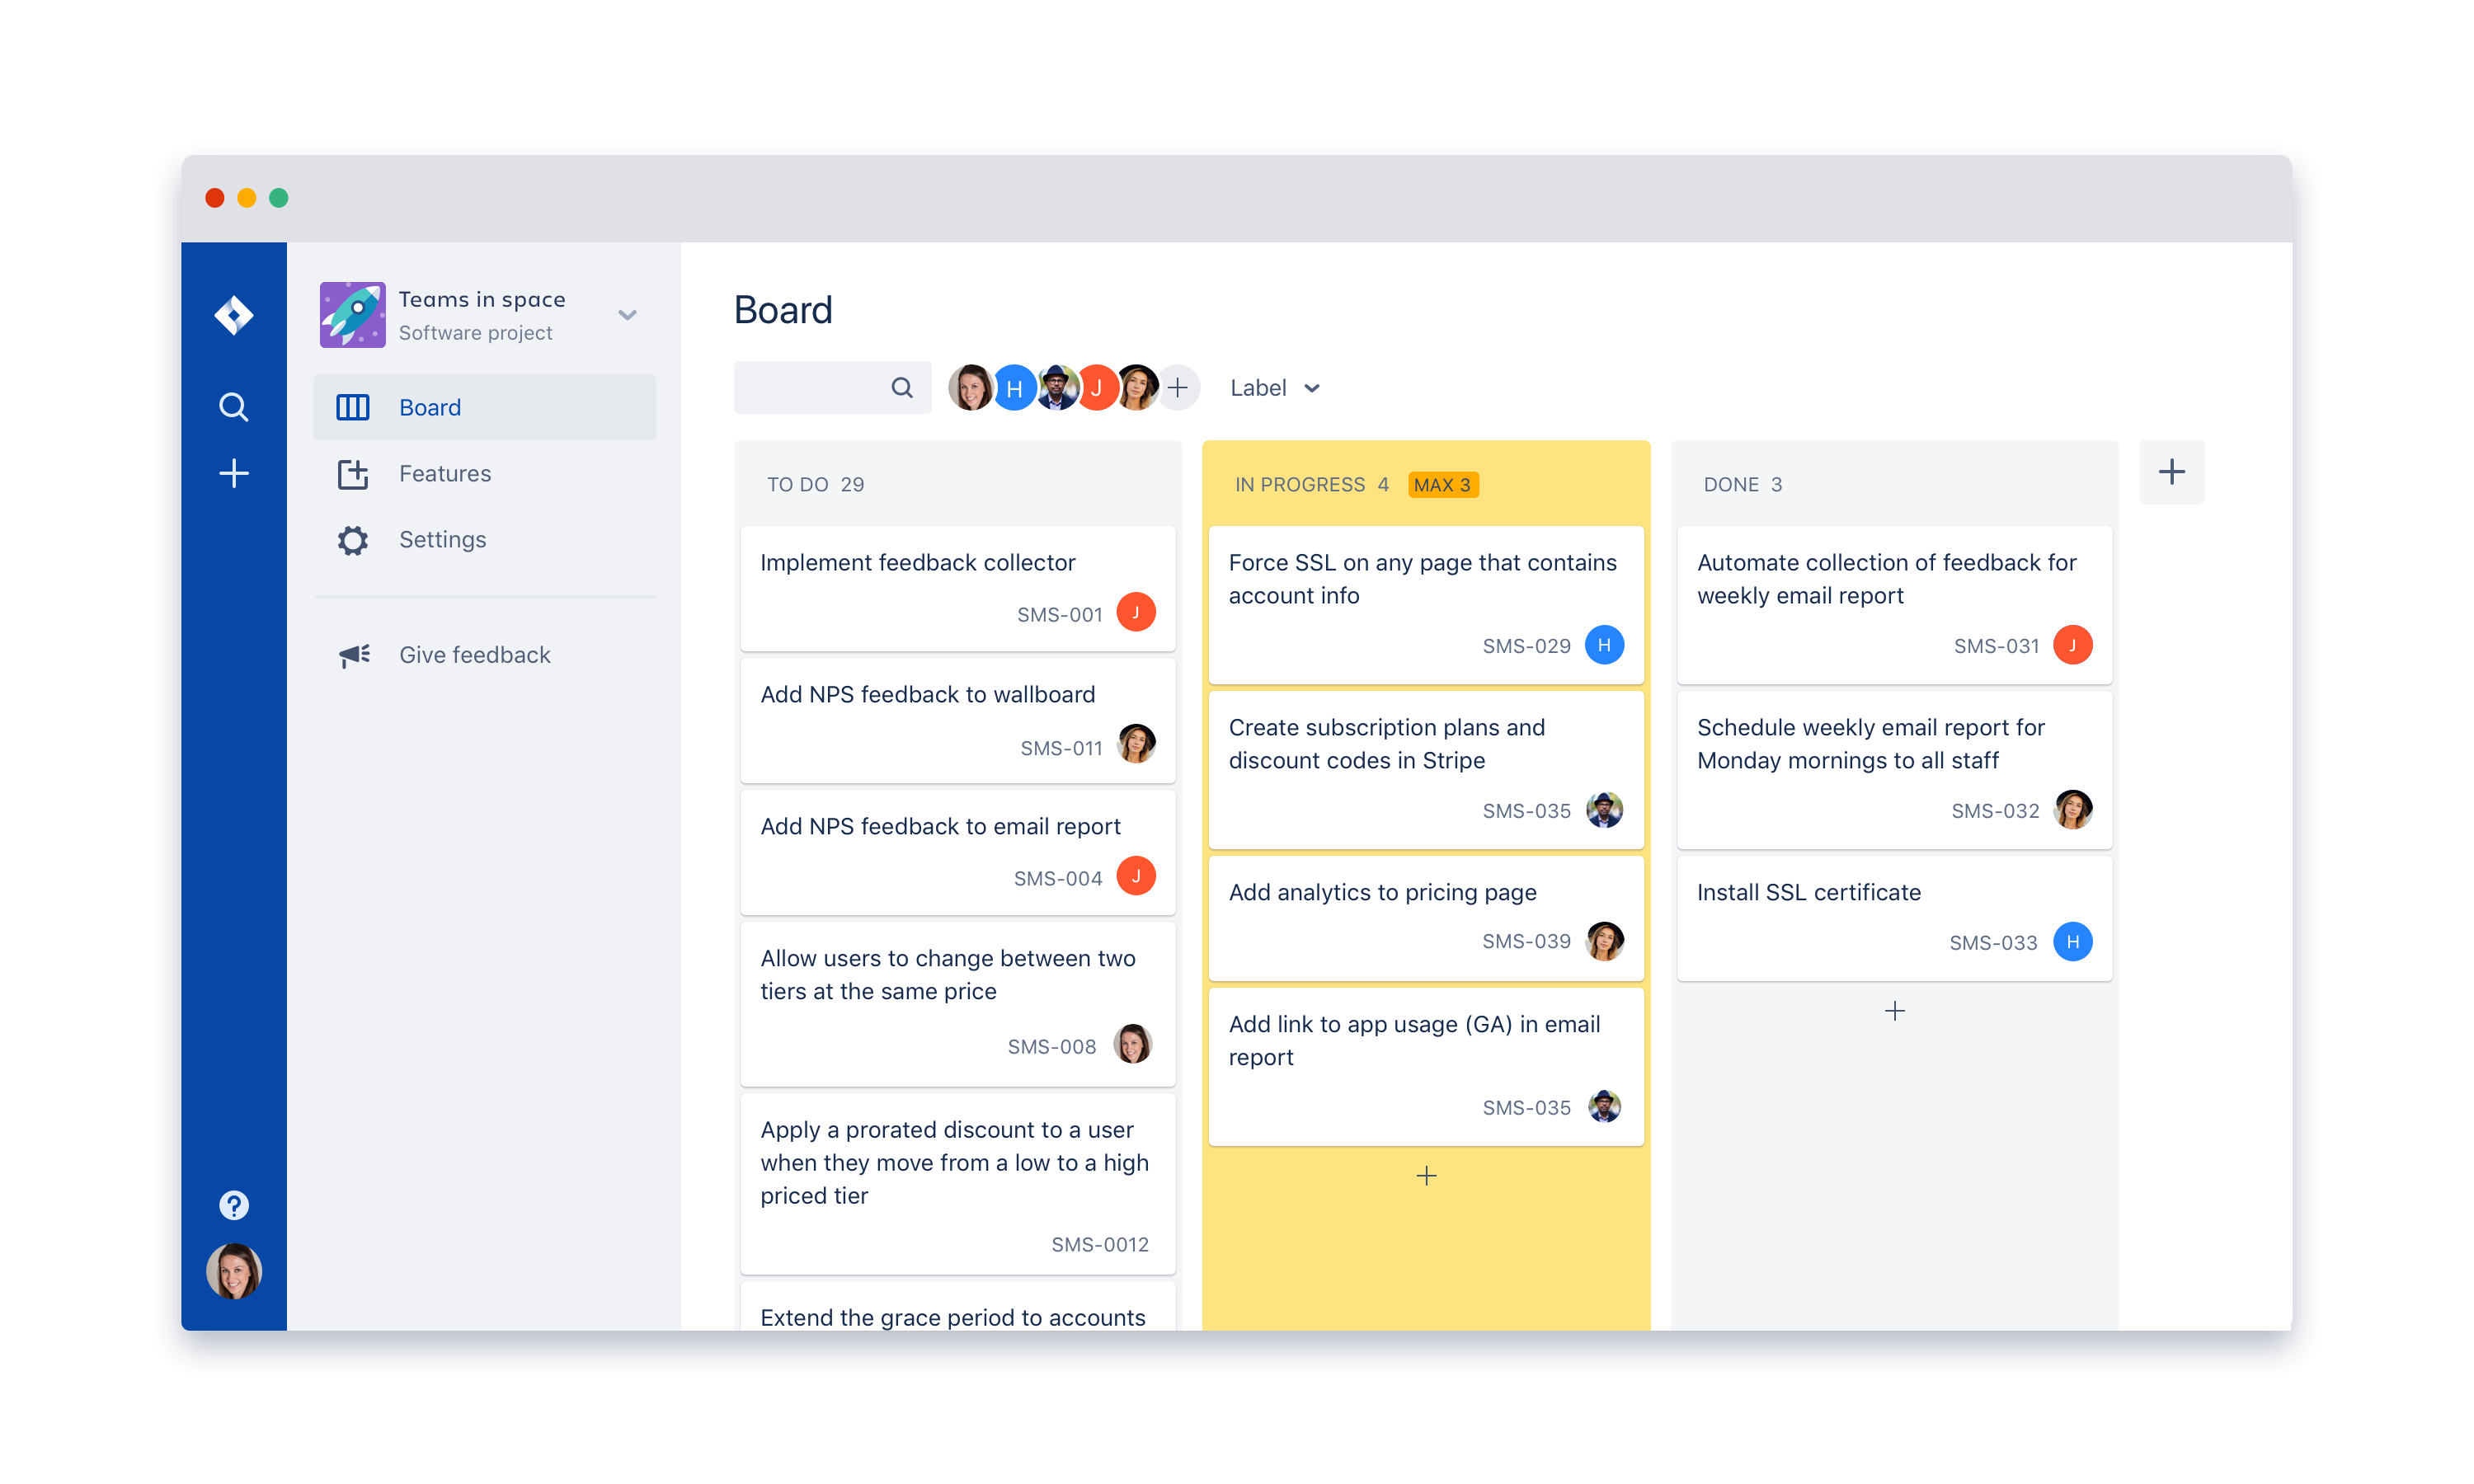
\includegraphics[width=1\textwidth]{Resources/kanban_board_example.png}
	\caption{Beispiel eines Kandan-Boards}
	\label{fig:kanban_board_example}
\end{figure}

Insgesamt bietet Kandan eine einfache und effektive Möglichkeit, den Fortschritt unseres Plotter-Projekts zu verwalten und sicherzustellen, dass wir kontinuierlich Verbesserungen vornehmen und auf unsere Ziele hinarbeiten.

\newpage

\subsection{Anwendung von Kanban}

Im Verlauf unseres Projekts haben wir uns für das Vorgehensmodell Kanban entschieden, um den Entwicklungsprozess zu organisieren und zu steuern. Kanban ist eine agile Methode, die auf kontinuierlicher Verbesserung und Flexibilität basiert. Es hilft, den Arbeitsfluss zu visualisieren, Engpässe zu identifizieren und die Produktivität des Teams zu steigern.

Wir haben ein Kanban-Board verwendet, um unsere Aufgaben und den Fortschritt im Projekt darzustellen. Unser Kanban-Board war in mehrere Spalten unterteilt, die den verschiedenen Phasen des Arbeitsablaufs entsprechen, z.B. 'To Do', 'In Progress', 'Review' und 'Done'. Jede Aufgabe wurde als Karte auf dem Board dargestellt, und wir haben die Karten zwischen den Spalten verschoben, um den Fortschritt der Aufgaben zu visualisieren.

Um den Entwicklungsprozess effektiv zu gestalten, haben wir unser Programm in kleinere Teile aufgeteilt, die wir Vorgänge (in Jira, dem von uns verwendeten Projektmanagement-Tool, genannt) nennen. Dies hat dazu beigetragen, dass wir uns auf bestimmte Aspekte der Anwendung konzentrieren und diese unabhängig voneinander entwickeln konnten.

In regelmäßigen Stand-up-Meetings haben wir den Status unserer Aufgaben überprüft, Engpässe identifiziert und die Prioritäten im Projekt angepasst. Dadurch konnten wir sicherstellen, dass die wichtigsten Aufgaben stets im Fokus standen und effektiv bearbeitet wurden.

\subsection{Vorteile und Erfahrungen}

Durch die Anwendung von Kanban in unserem Projekt haben wir verschiedene Vorteile erfahren:

\begin{itemize}
\item \textbf{Flexibilität}: Kanban hat es uns ermöglicht, schnell auf Änderungen im Projektumfeld oder in den Anforderungen zu reagieren. Dadurch konnten wir unsere Prioritäten anpassen und sicherstellen, dass wir uns auf die wichtigsten Aspekte des Projekts konzentrierten.
\item \textbf{Transparenz}: Durch die Visualisierung des Arbeitsablaufs auf dem Kanban-Board konnten alle Teammitglieder den aktuellen Status der Aufgaben und den Fortschritt des Projekts einsehen. Dies hat zu einer besseren Kommunikation und Zusammenarbeit im Team geführt.
\item \textbf{Effizienz}: Die Anwendung von Kanban und die Aufteilung des Programms in kleinere Vorgänge haben dazu beigetragen, Engpässe im Arbeitsablauf zu identifizieren und zu beseitigen. Dies hat die Produktivität des Teams gesteigert und dazu geführt, dass Aufgaben schneller und effizienter abgeschlossen wurden.
\item \textbf{Kontinuierliche Verbesserung}: Die regelmäßigen Stand-up-Meetings und die Möglichkeit, den Arbeitsablauf anzupassen, haben dazu beigetragen, kontinuierliche Verbesserungen im Projektprozess zu fördern. Dadurch konnten wir mögliche Probleme frühzeitig erkennen und Lösungen entwickeln, um diese zu beheben.
\end{itemize}

\newpage

Insgesamt hat die Anwendung von Kanban in unserem Projekt dazu beigetragen, einen effizienten und flexiblen Entwicklungsprozess zu gestalten, der es uns ermöglichte, eine erfolgreiche und benutzerfreundliche Anwendung zu entwickeln.

\section{Anforderungsanalyse}

\subsection{Funktionale Anforderungen}

\subsection{Nicht funktionale Anforderungen}

\subsection{Aktivitätsdiagramm}

\newpage

\section{Use-Case-Diagramm}

\subsection{Erklärung}

Das Use-Case-Diagramm beschreibt die Funktionalität des Plotters und zeigt, wie Benutzer mit der Anwendung interagieren können. Der Benutzer kann in ein Textfeld seine gewünschte Funktion eingeben und mithilfe von Buttons Sonderzeichen in das Textfeld schreiben. Der Benutzer hat auch die Möglichkeit, verschiedene Buttons zu verwenden, um die Funktion zu bearbeiten, wie zum Beispiel die Sichtbarkeit, Ableitung, Kurvendiskussion oder die Funktion zu löschen. Zusätzlich kann der Benutzer den Anzeigebereich der Funktion mithilfe von Zoomen oder Verschieben verändern.

\subsection{Diagramm}

Das folgende Diagramm zeigt das Use-Case-Diagramm für unseren Plotter:

\begin{figure}[h]
\centering
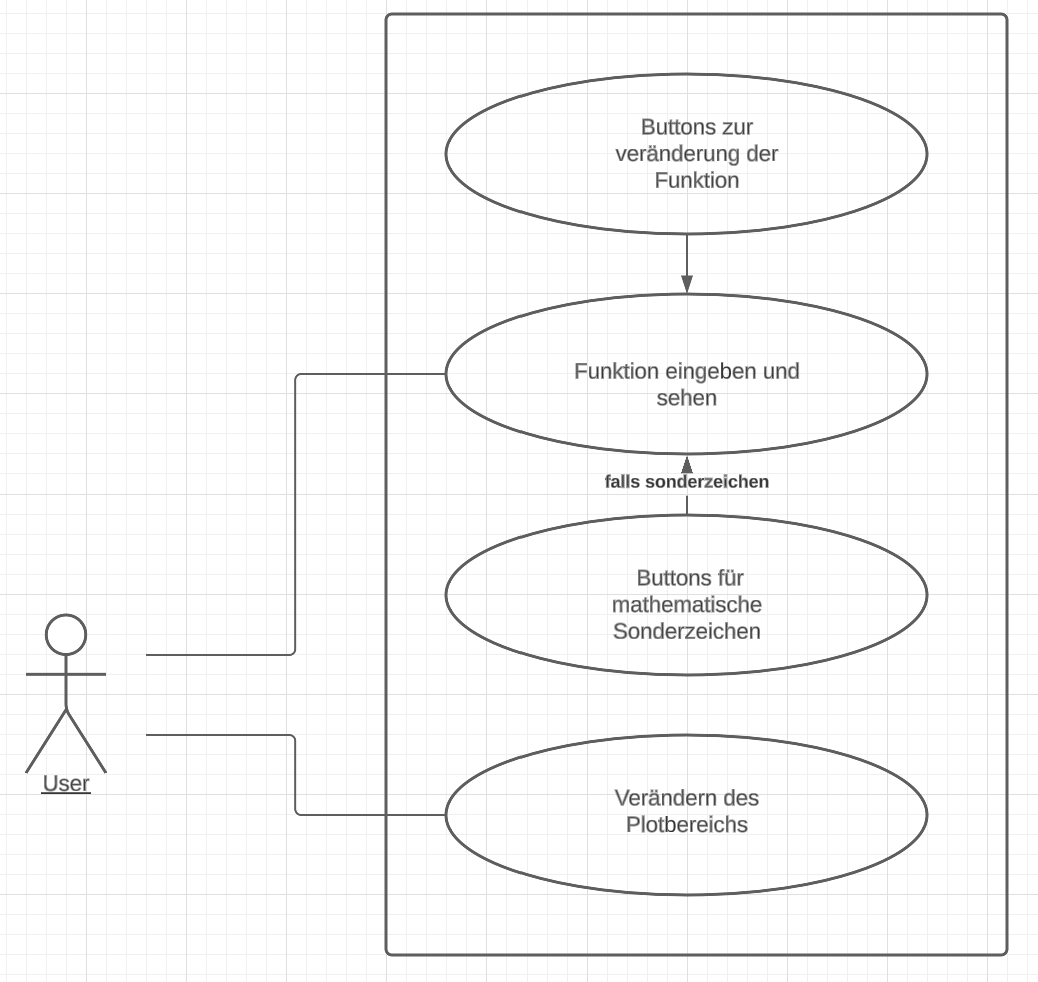
\includegraphics[width=0.8\textwidth]{Resources/use-case-diagram.png}
\caption{Use-Case-Diagramm des Plotters}
\label{fig:use_case_diagram}
\end{figure}

Das Diagramm veranschaulicht die verschiedenen Aktionen, die ein Benutzer ausführen kann, um mit der Anwendung zu interagieren und mathematische Funktionen zu visualisieren und zu analysieren.

\section{Systemarchitektur}

\subsection{Übersicht}

\subsection{Frontend}

\subsection{Backend}

\subsection{Klassendiagramm}

\section{Umsetzung (Programmierung)}

\subsection{Backend-Entwicklung}

\subsection{Frontend-Entwicklung}

\subsubsection{UI-Prototyp}

\subsection{Integration von APIs}

\subsection{Teststrategie}

\section{Benutzung (User Guide)}

\subsection{Installation und Einrichtung}

\subsection{Bedieung der Anwendung}

\subsection{Beispiele}

\section{Fazit}

\subsection{Zusammenfassung}

\subsection{Erreichte Ziele}

\subsection{Zukünftige Erweiterungen}

\section{Anhang}

\subsection{Arbeitstagebuch (Planung)}

\subsection{Arbeitstagebuch (Umsetzung)}

\subsection{Quellcode}

\subsection{Screenshots}

\subsection{Lizenzinformationen}


\end{document}